\documentclass[english]{article}
\usepackage[T1]{fontenc}
\usepackage[utf8]{inputenc}
\usepackage{babel}
\usepackage[unicode=true,pdfusetitle,
 bookmarks=true,bookmarksnumbered=false,bookmarksopen=false,
 breaklinks=true,pdfborder={0 0 1},backref=false,colorlinks=false]
 {hyperref}
\usepackage{tabularx}
\usepackage{graphicx}
\graphicspath{{images/}}
\usepackage{svg}
\usepackage{float}
\usepackage{titling}
\renewcommand{\arraystretch}{1.4}
\usepackage{listings}
\usepackage{color}
\definecolor{javared}{rgb}{0.6,0,0} % for strings
\definecolor{javagreen}{rgb}{0.25,0.5,0.35} % comments
\definecolor{javapurple}{rgb}{0.5,0,0.35} % keywords
\definecolor{javadocblue}{rgb}{0.25,0.35,0.75} % javadoc

\lstset{language=Java,
	basicstyle=\ttfamily\small,
	keywordstyle=\color{javapurple}\bfseries,
	stringstyle=\color{javared},
	commentstyle=\color{javagreen},
	morecomment=[s][\color{javadocblue}]{/**}{*/},
	numbers=left,
	numberstyle=\tiny\color{black},
	stepnumber=1,
	numbersep=10pt,
	tabsize=4,
	showspaces=false,
	showstringspaces=false,
	linewidth=17cm,
	breaklines=true
	}

\pretitle{%
	\begin{center}
		\LARGE
		
\includegraphics[width=250pt]{../other/Logo_blu.png}\\[\bigskipamount]~\\[\bigskipamount]
	}
\posttitle{\end{center}}

\begin{document}

\title{Politecnico di Milano\\
 A.A. 2016–2017 \\
Software Engineering 2: “PowerEnJoy” \\
\emph{Design Document}}

\author{Pietro Ferretti, Nicole Gervasoni, Danilo Labanca}
%\date{December 11, 2016}
\maketitle

\newpage

\tableofcontents{}

\newpage

\section{Introduction}

\subsection{Purpose}

\paragraph{}
The purpose of this document is to specify in a more technical way how our system is designed to be built and work. 
This document is intended for developers, designers and all interested stakeholders as a guideline for the implementation of the system.

\paragraph{}
This document will first of all illustrate the system architecture, the components that make it up and how each of its components is designed to interact with each other.

Furthermore this document will describe the behaviour of the system and the applications, from both the back-end and the front-end side.

Finally this document will describe the patterns we used to design the system and how each of them comes into play.

%% magari ridurre a due righe ^^^


\subsection{Scope}
\paragraph{}
The aim of this project is to specify in detail a new digital management software for PowerEnJoy, a car-sharing service that employs electric cars only.
%
%\paragraph{}
PowerEnjoy will offer a very valuable service to its users, letting them borrow cars to drive around the city freely, as an alternative to their own vehicles and public transport.
%Among the advantages of using PowerEnJoy we can note being able to find available cars in any place that is served by our system and having dedicated spots to park in (namely, PowerEnJoy's power grid stations). 
%Furthermore, thanks to the fact that all the cars that we provide are electrically powered, PowerEnJoy is also very environmentally friendly.

\paragraph{}
PowerEnJoy's users, after registering, will be able to reserve, unlock and drive the cars our system will provide. Users will be charged per minute until they park the car in a safe area and end the ride.
Users will be able to park their car temporarily and use it again later, or end their ride remotely.

Our system will incentivize virtuous behaviour by offering several discounts if certain conditions are met (like charging a car at a power grid station).


\newpage
\subsection{Definitions, Acronyms, Abbreviations}

% vanno tolte le definizioni che non vengono usate in questo documento
% e aggiunte quelle in più

\subsubsection{Definitions}

\begin{itemize}
\item{\textit{Guest}: a person that is not registered to the system.}
\item{\textit{User}: a person that is registered to the system. Users can log in to the system with their email or username and their password. Their first name, last name, date of birth, driving license ID are stored in the database.}
\item{\textit{Safe area}: a location where the user can park and leave the car. Users can end their ride and park temporarily only in these locations. The set of safe areas is predefined by the system.}
\item{\textit{Power grid station}: a place where cars can be parked and plugged in. While a car is plugged in a power grid station its battery will be recharged. Power grid stations are by definition safe areas.}
\item{\textit{Available car}: a car that is currently not being used by any user, and has not been reserved either. Available cars are in good conditions (not dirty nor damaged) and don’t have dead batteries.}
\item{\textit{Reservation}:
	\begin{itemize}
		\item{the operation of making a car reserved for a user, i.e. giving permission to unlock and use the car only for that user, forbidding reservations by other users.}
		\item{the time period between the moment a reservation is requested and the moment the user unlocks the car, or the reservation is canceled.}
	\end{itemize}
}
\item{\textit{Ride}: the time period from the moment a reserved car is unlocked to the moment the user notifies that he wants to stop using the car and closes all the doors. A ride doesn’t stop when a car is temporarily parked, but continues until the user chooses to leave the car definitely.}
\item{\textit{Possession}: users that have reserved and unlocked a car are said to have possession of the car. While a user has possession of a car they are the only person that can drive it, lock or unlock it, and no other person can take possession of it until the user frees it. Users lose possession of a car when their ride ends.}
\item{\textit{Temporary parking}: the act of parking a car in a safe area and, after notifying the system, locking it and leaving it for a finite amount of time. The user that does this retains the right to use the car and can unlock it later to use it again.}
\item{\textit{Bill}: a record of the money owed by the user at the end of a ride.}
\item{\textit{Outstanding bill}: a bill that hasn’t been paid yet. }
\item{\textit{Suspended user}: a user that cannot reserve or use cars. Usually users are suspended because they have outstanding bills.}
\item{\textit{Payment method}: a way to transfer money from the user to the system. Our system will only accept credit cards and online accounts like Paypal.}
\item{\textit{Payment API}: an interface to carry out money transactions, offered by the external provider associated to the payment method used (e.g. a bank).}
\item{\textit{CAN bus}: a vehicle bus standard designed to allow micro controllers and devices to communicate with each other.}
\end{itemize}

\subsubsection{Acronyms}
\begin{itemize}
\item{\textbf{DD}: Design Document}
\item{\textbf{RASD}: Requirements Analysis and Specification Document}
\item{\textbf{DB}: Database}
\item{\textbf{CVV}: Card Verification Value}
\item{\textbf{DOB}: Date of birth}
\item{\textbf{PGS}: Power Grid Station}
\item{\textbf{GPS}: Global Positioning System}
\item{\textbf{CAN bus}: Controller Area Network bus}
\end{itemize}

\subsubsection{Abbreviations}
\begin{itemize}
\item{\textbf{[Gx]}: Goal}
\item{\textbf{[RE.x]}: Functional Requirement}
\item{\textbf{[UC.x]}: Use Case}
\end{itemize}

\subsection{Reference Documents}

\begin{itemize}
	\item{IEEE Std. 1016-2009, “IEEE Standard for Information Technology -- Systems Design -- Software Design Descriptions”}
	\item{ISO/IEC/IEEE Std. 42010:2011, “Systems and software engineering -- Architecture Description”}
	\item{Specification document: “Assignments AA 2016-2017.pdf”}
\end{itemize}

\newpage{}

\subsection{Document Structure}

%% DA RILEGGERE

This document is structured as follows:
\begin{itemize}
\item{\textbf{Section 1 -- Introduction:} this section introduces the design document. It contains
	a justification of his utility and indications on which parts are covered in
	this document that are not covered by the RASD.}
\item{\textbf{Section 2 -- Architectural Design:} this section is divided into more parts:
	\begin{itemize}
		\item{\textbf{Overview:} this section shows a high-level view of our system's architecture.}
		\item{\textbf{Component View:} this section gives a more detailed (in-depth) view of the components of the application and how they communicate.}
		\item{\textbf{Deployment View:} this section shows the way the components will be deployed to run our application.}
		\item{\textbf{Runtime View:} in this section we use sequence diagram to show the flow of the most important functionalities of the system.}
		\item{\textbf{Component Interfaces:} the interfaces between the components are presented in this section.}
		\item{\textbf{Selected Architectural Styles and Patterns:} this section explains the architectural choices taken during the creation of the application.}
		\item{\textbf{Other Design Decisions}}
	\end{itemize}}
\item{\textbf{Section 3 -- Algorithm Design:} this section describes the most critical parts via some algorithms. Pseudo code is used in order to hide unnecessary implementation details in order to focus on the most important parts.}
\item{\textbf{Section 4 -- User Interface Design:} this section presents mockups and user experience explained via UX and BCE diagrams.}
\item{\textbf{Section 5 -- Requirements Traceability:} this section aims to explain how the requirements identified in the RASD are linked to design elements.}
\item{\textbf{Effort Spent} }
\item{\textbf{References} }
\item{\textbf{Revisions} }
\end{itemize}

\newpage

\section{Architectural Design}

\subsection{Overview}

\subsection{Component View}

% inserire immagine component view
\begin{figure}[H]
	\centering
	\makebox[\textwidth][c]{
		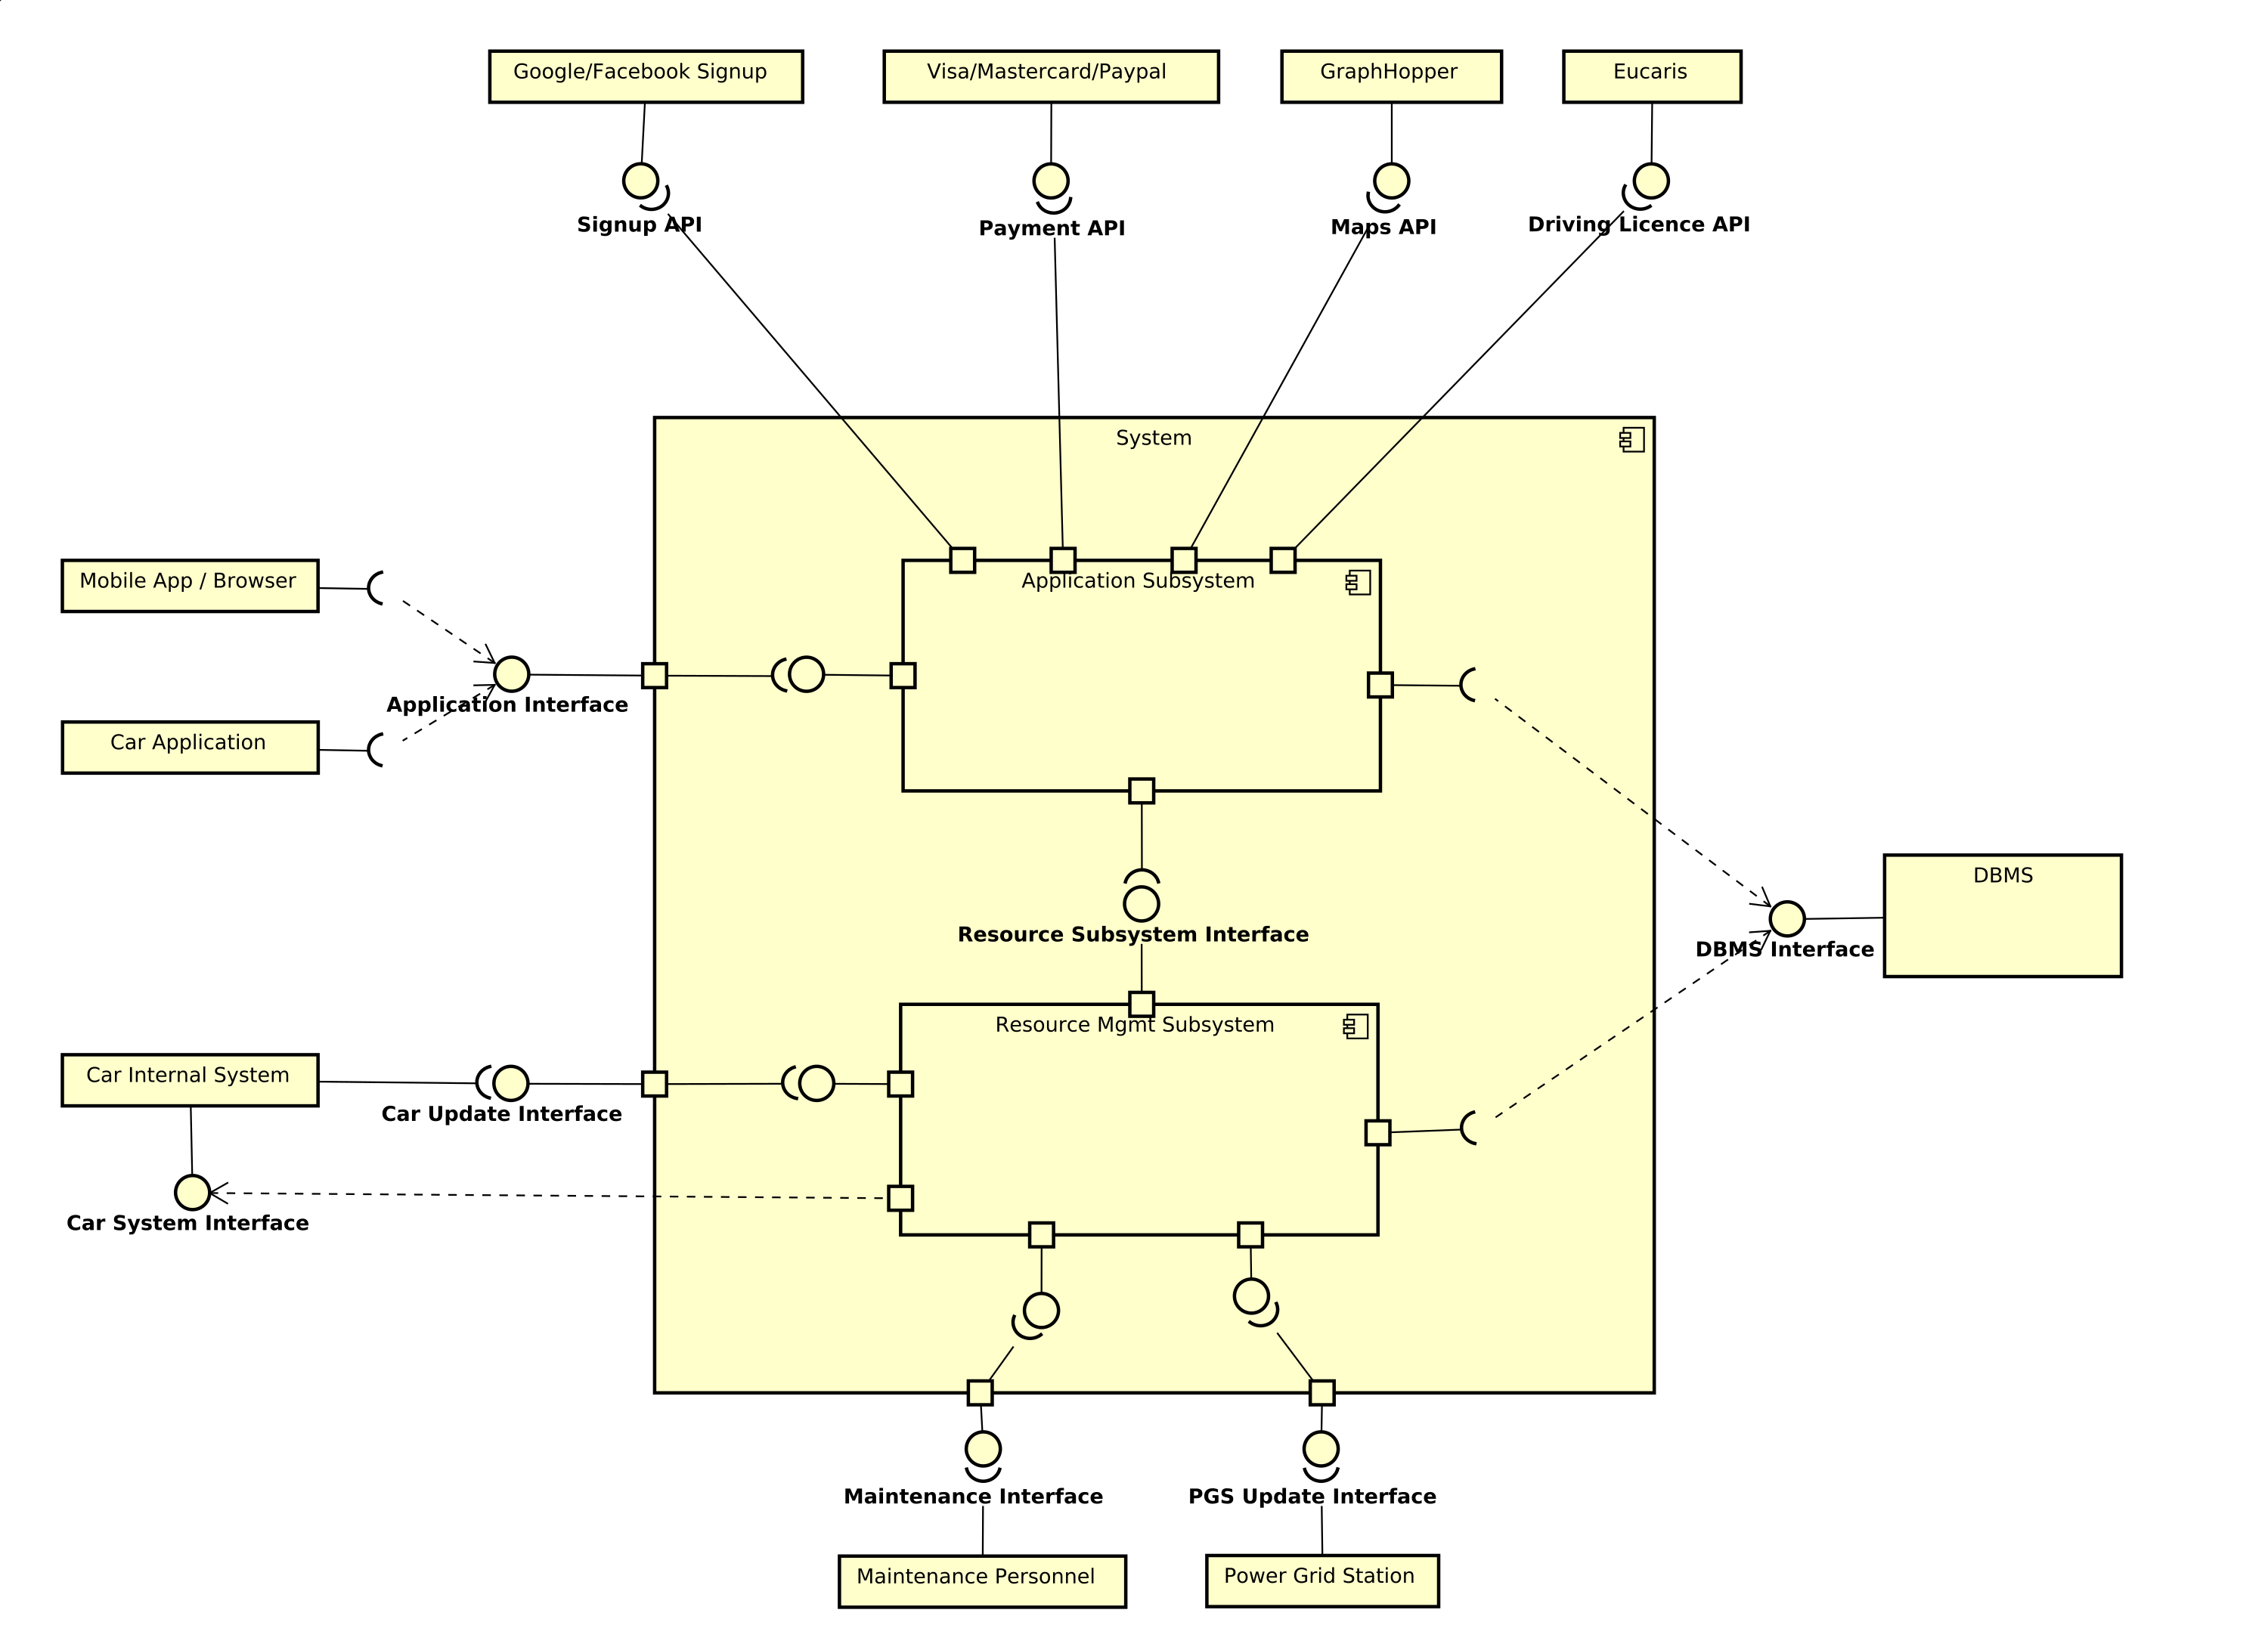
\includegraphics[width=450pt]{comp_1.png}
	}
	\caption{Component Diagram Overview}
	\label{componentdiagram1}
\end{figure}
\begin{figure}[H]
	\centering
	\makebox[\textwidth][c]{
		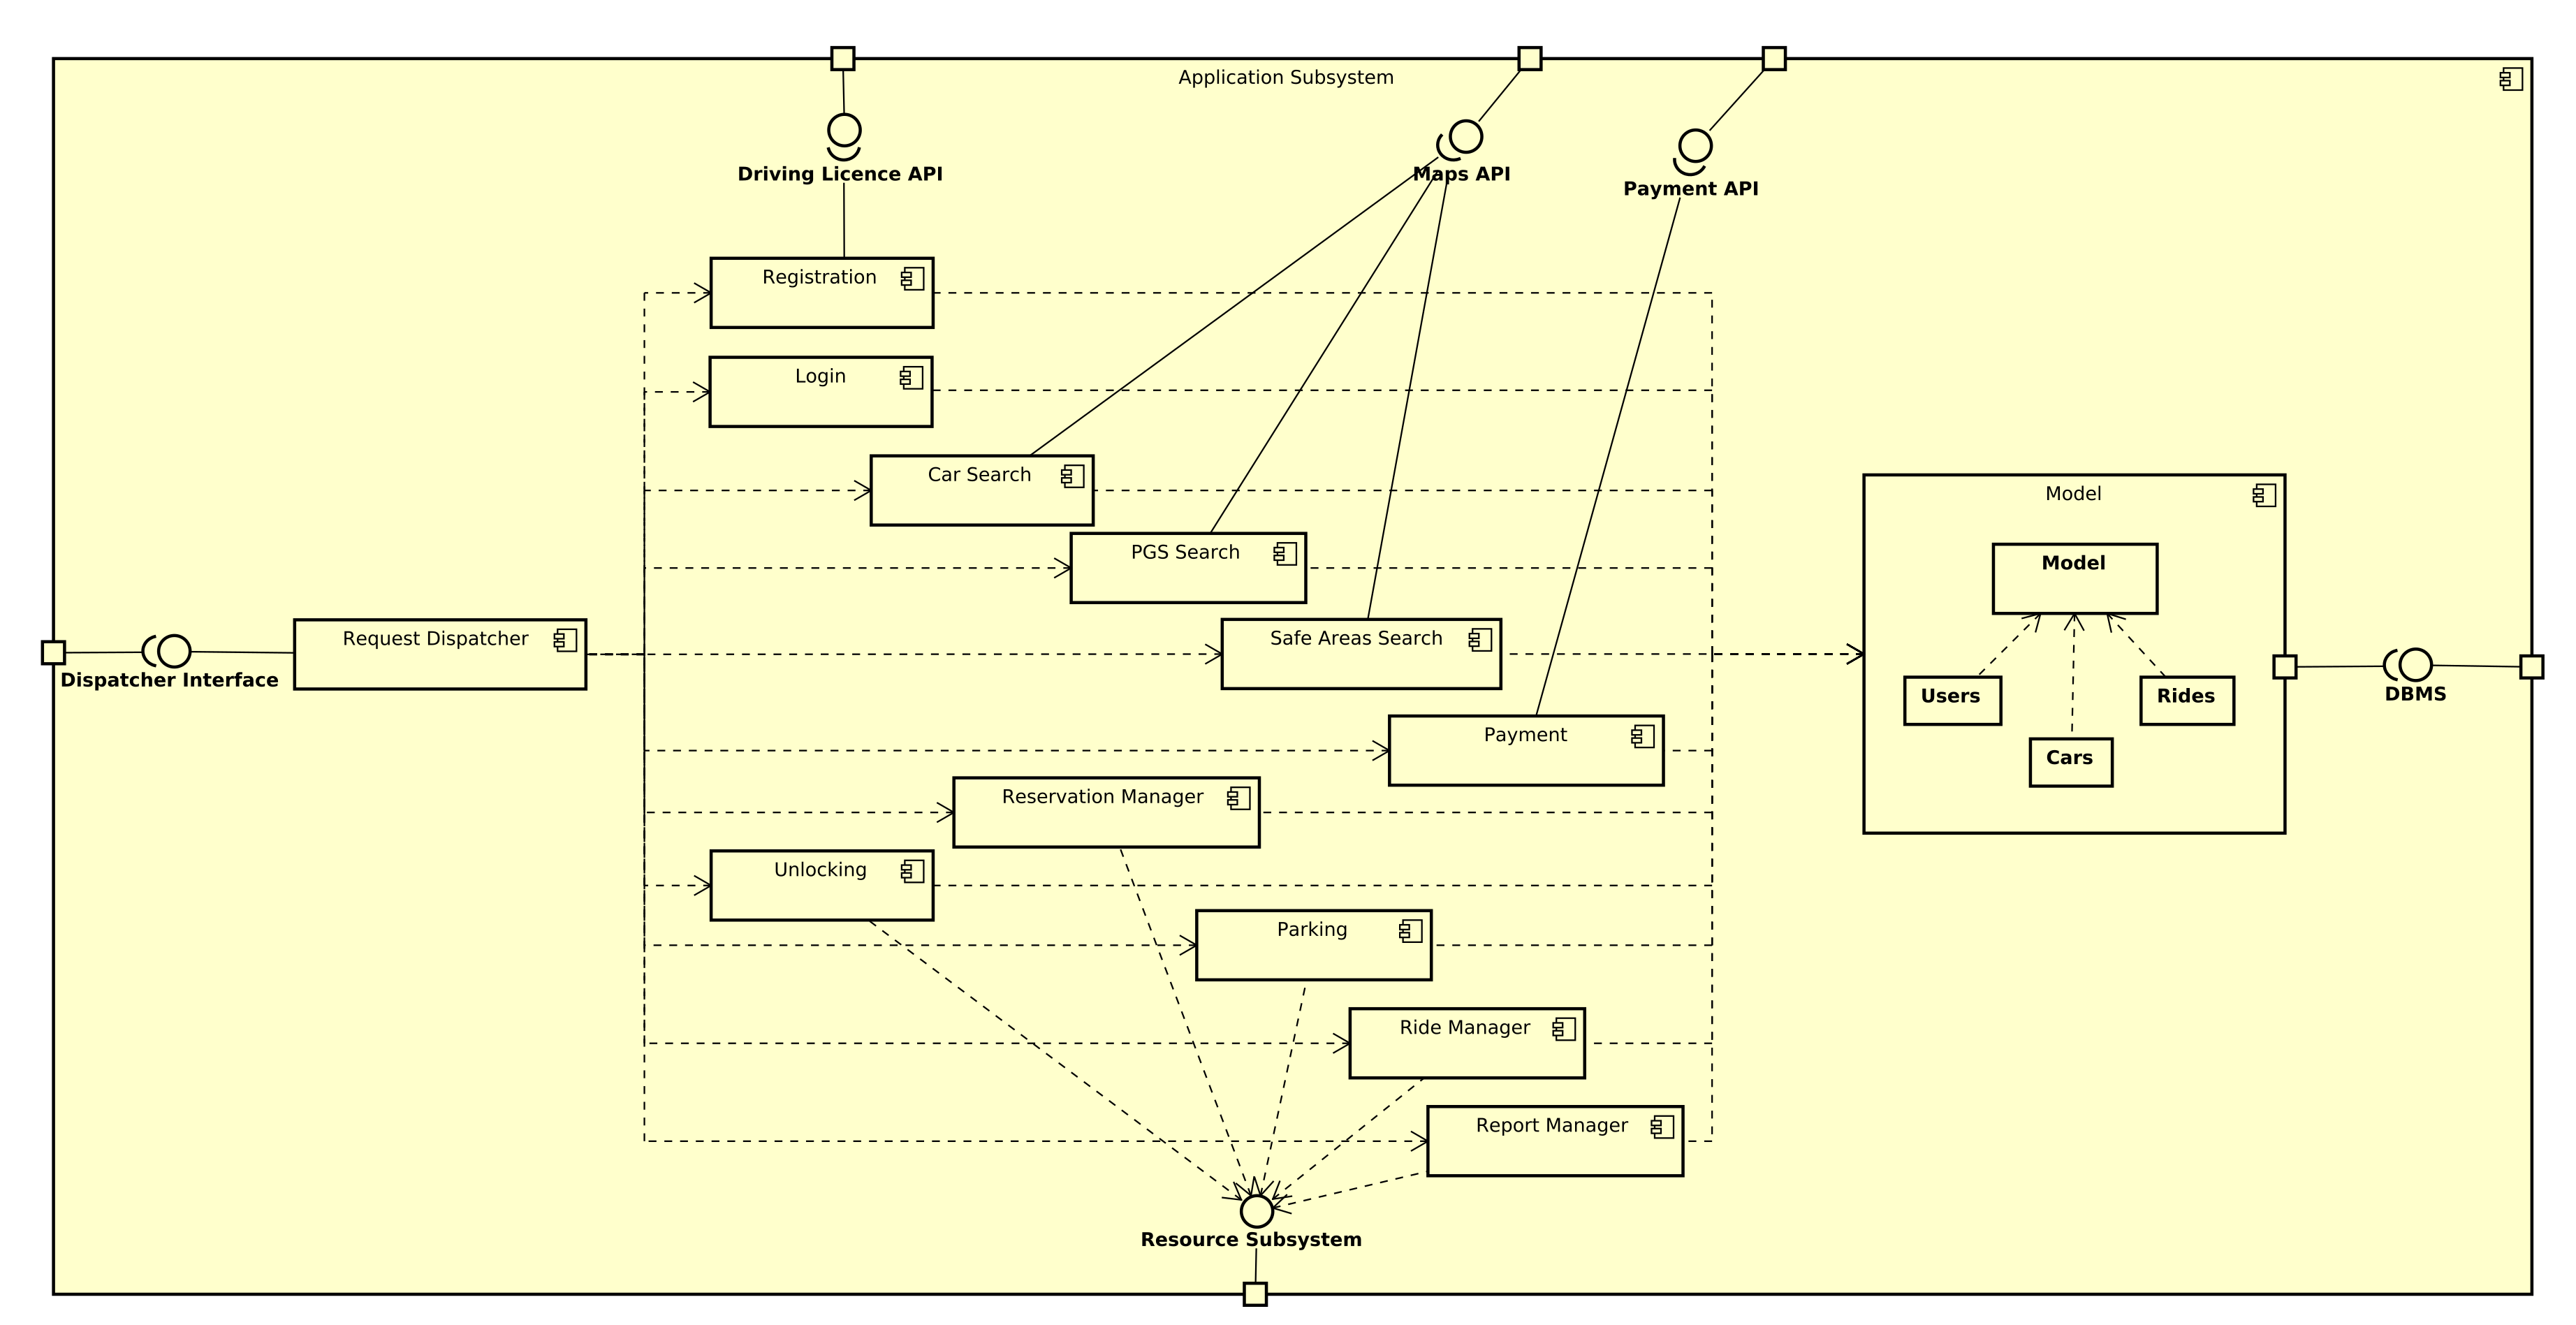
\includegraphics[width=450pt]{comp_2.png}
	}
	\caption{Component Diagram for the Application Subsystem}
	\label{componentdiagram2}
\end{figure}
\begin{figure}[H]
	\centering
	\makebox[\textwidth][c]{
		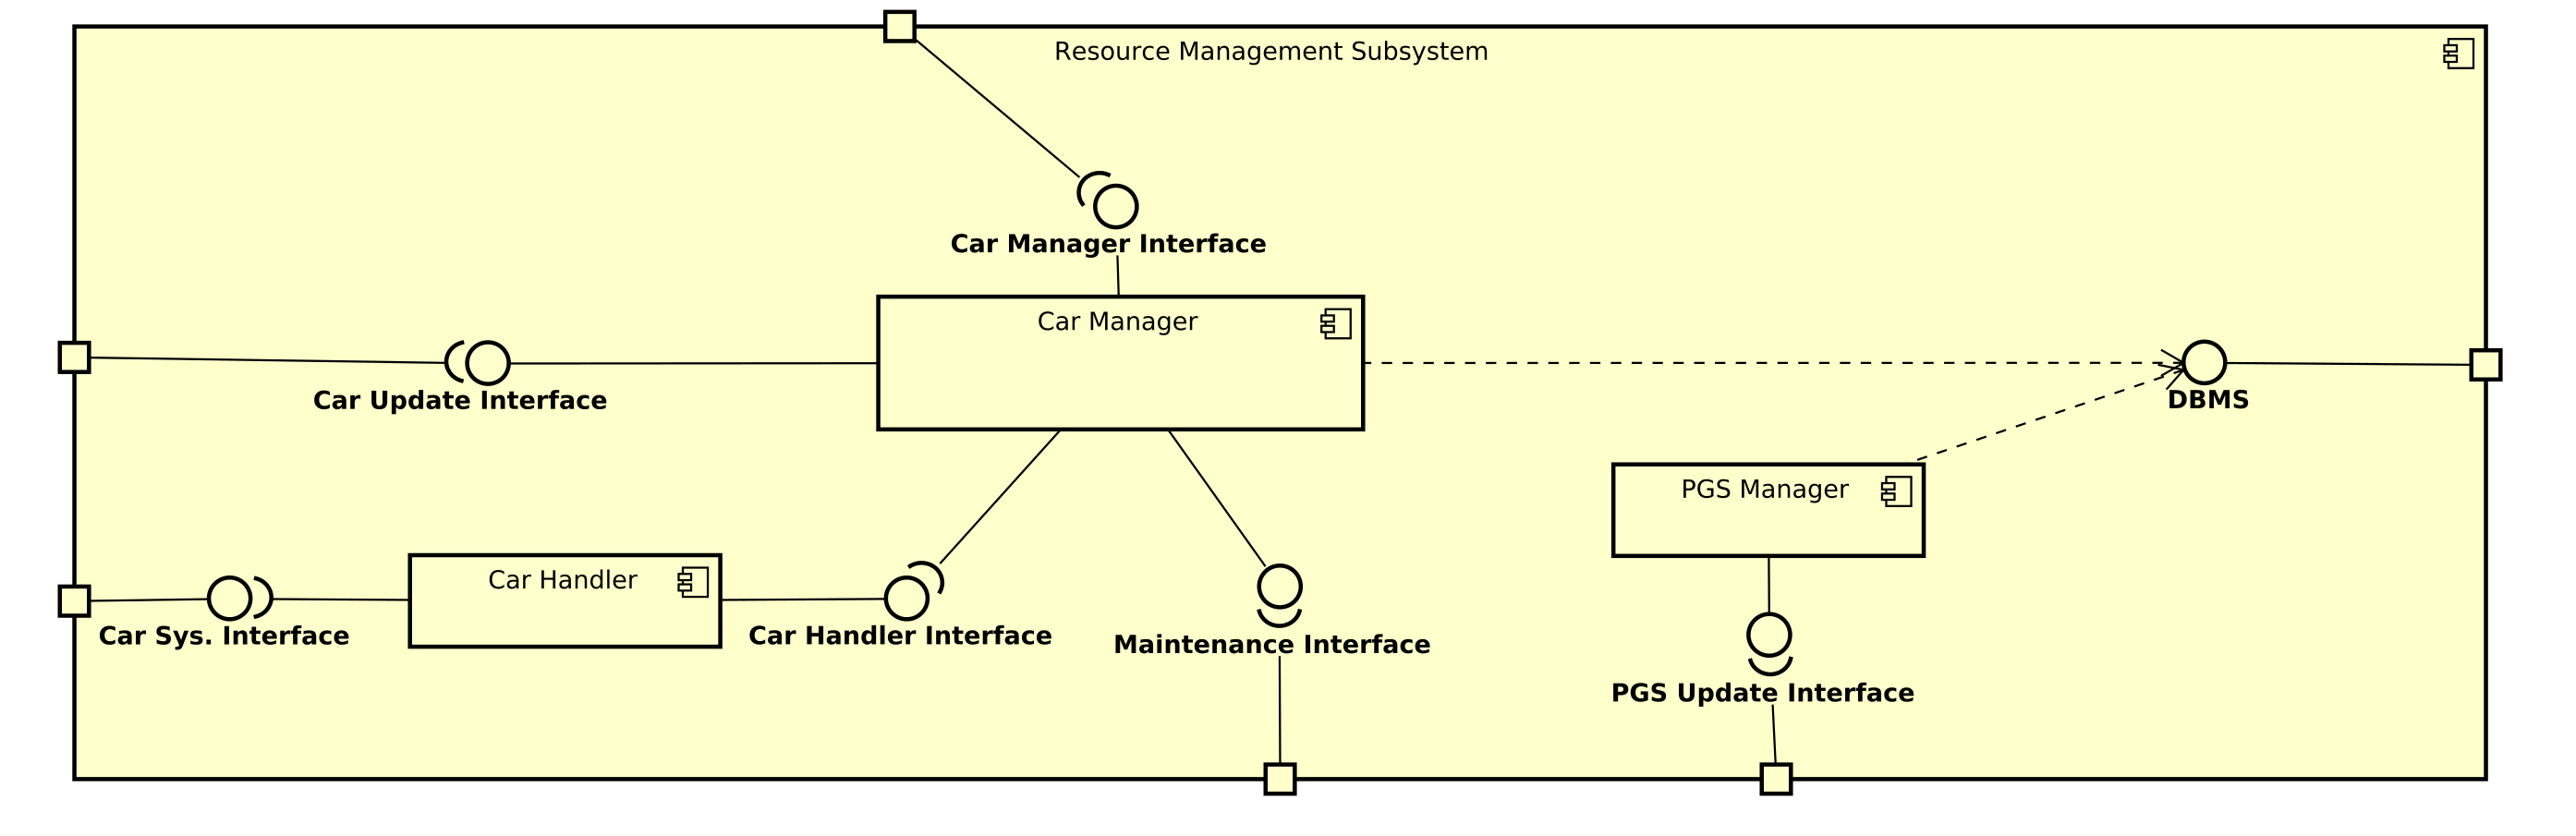
\includegraphics[width=400pt]{comp_3.png}
	}
	\caption{Component Diagram for the Resource Management Subsystem}
	\label{componentdiagram3}
\end{figure}
% spiegazione veloce immagine

\newpage
\subsection{Deployment View}

% inserire immagine deployment view
\begin{figure}[H]
	\centering
	\makebox[\textwidth][c]{
		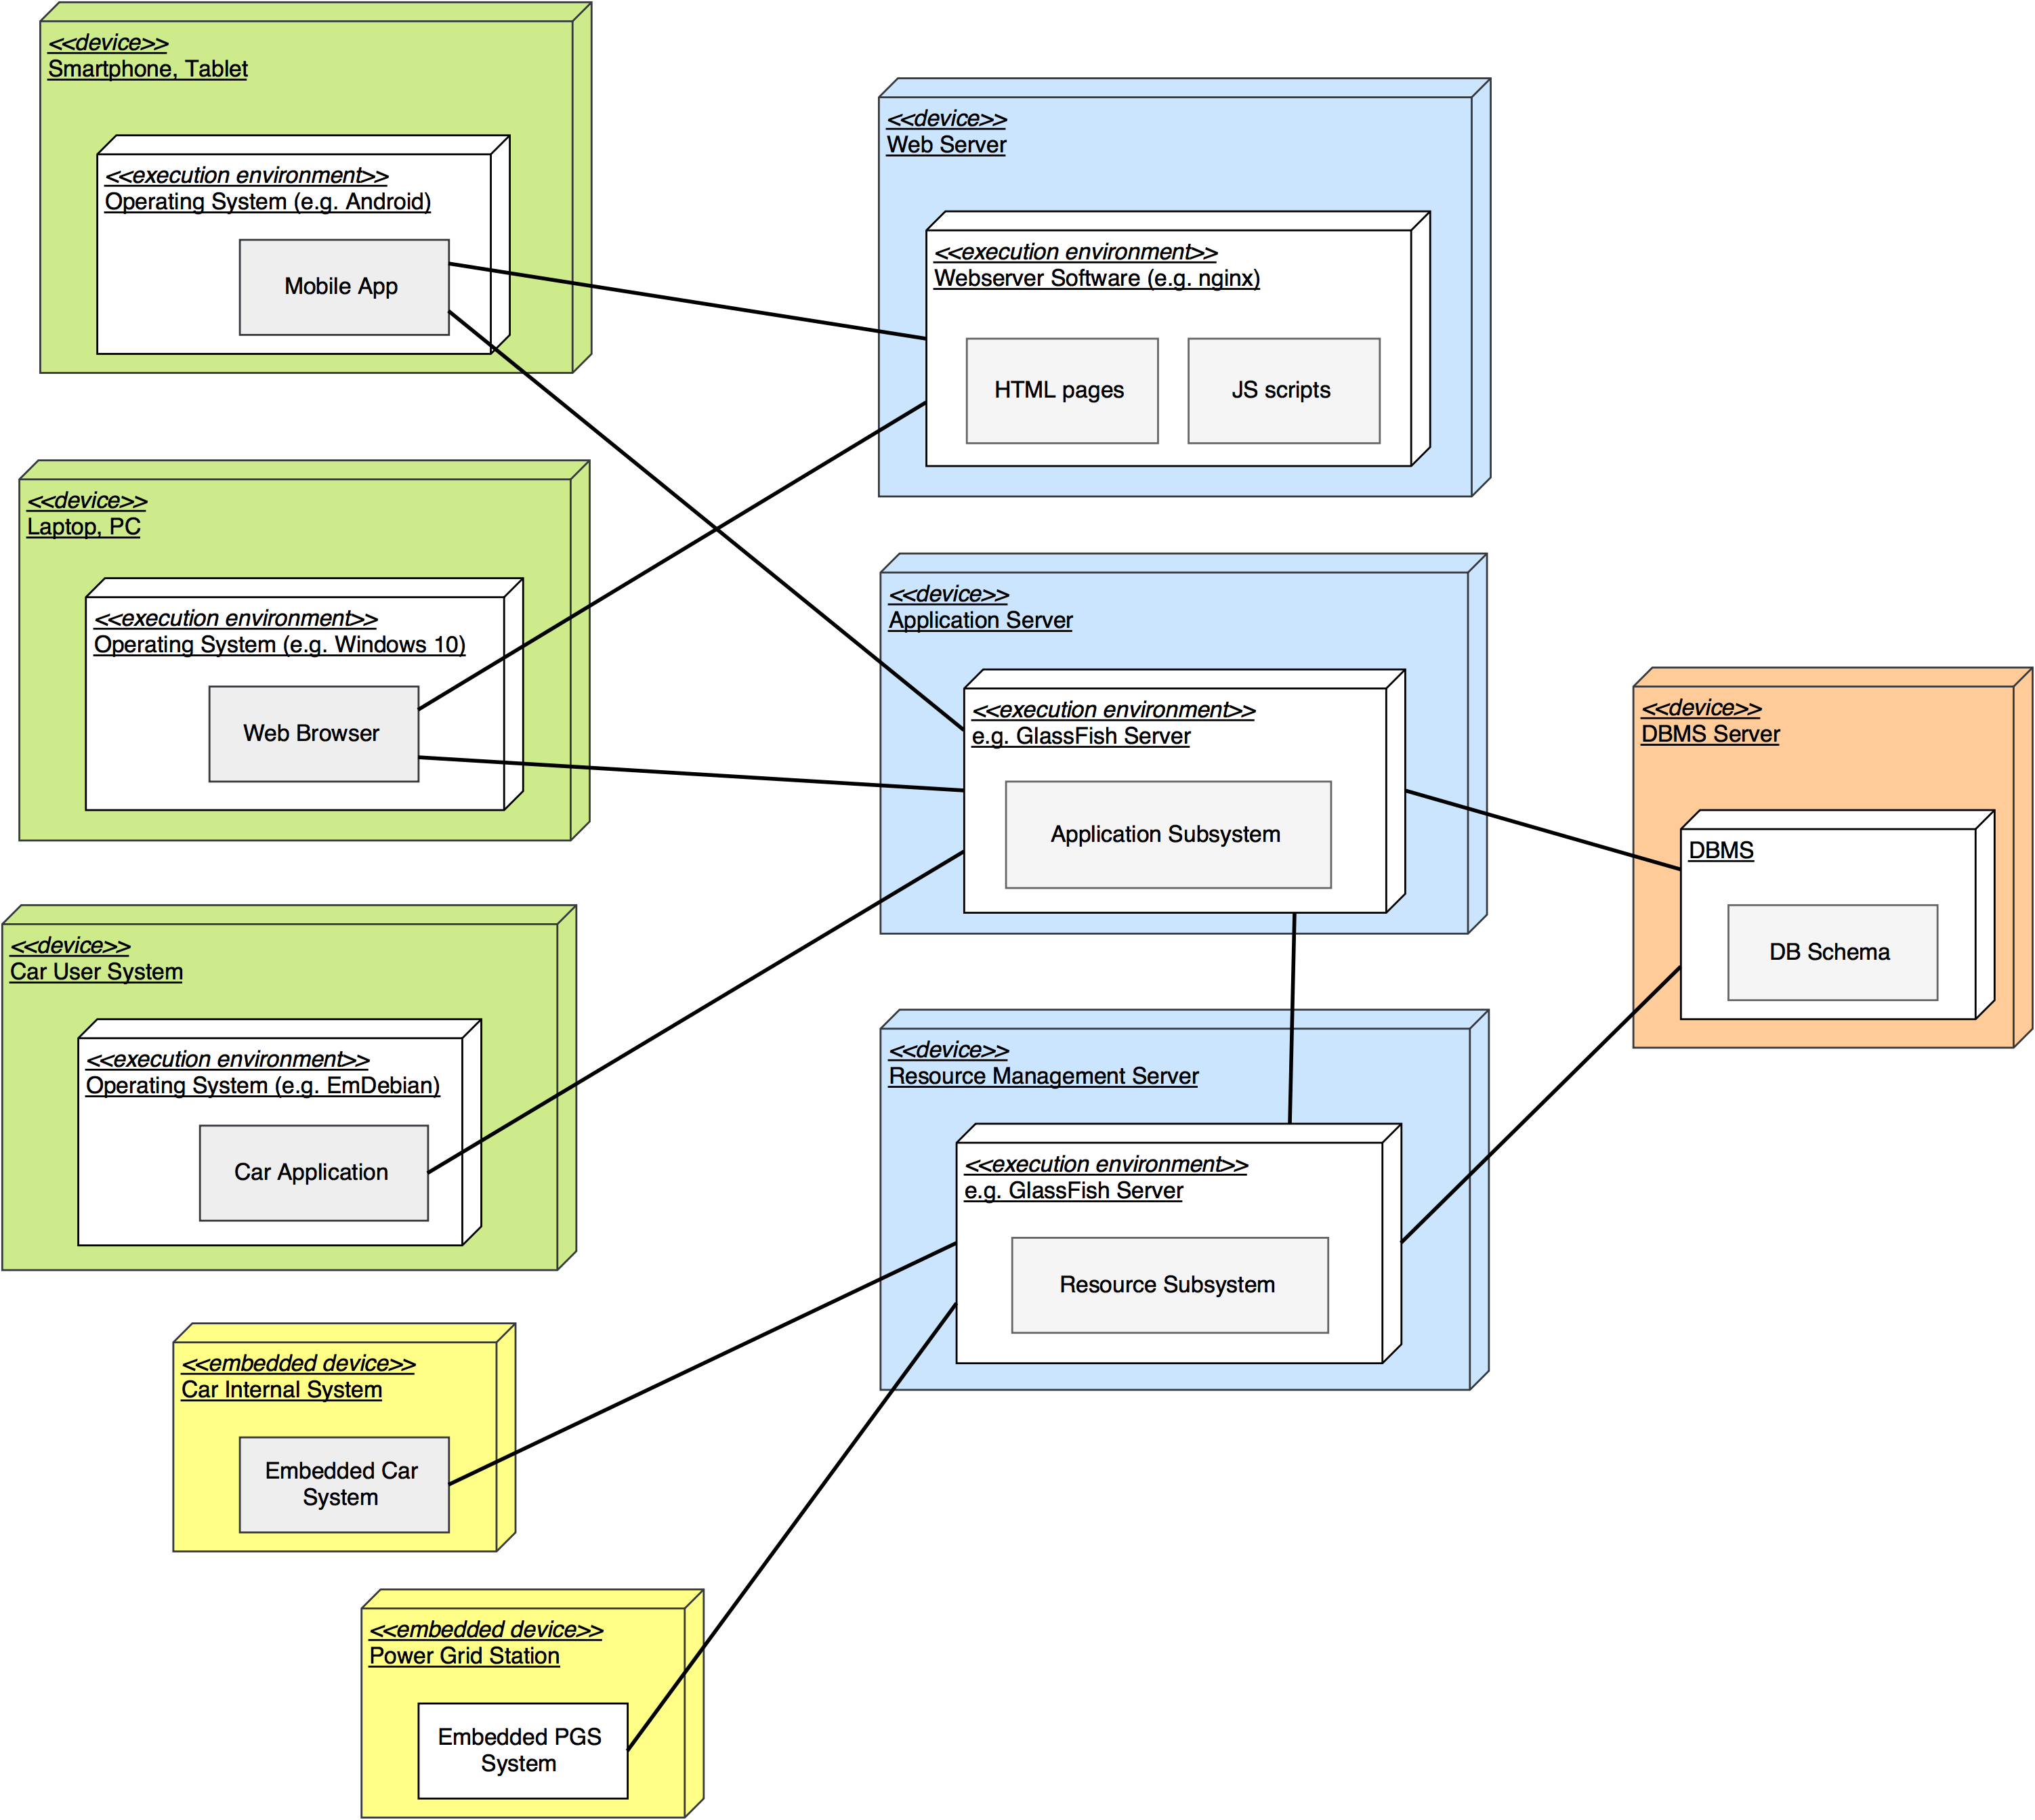
\includegraphics[width=450pt]{deployment_diagram.png}
	}
	\caption{Deployment Diagram}
	\label{deploymentdiagram}
\end{figure}

% spiegazione veloce immagine
tre tier: client, business logic, database

client:
- app e browser si collegano al web server per avere le pagine web, poi si collegano all'application server per raccogliere i dati
- l'applicativo sulla macchina non è basato sul web e si collega direttamente all'application server per avere tutto
- esiste un "resource management server" che raccoglie informazioni (gps, ecc.) dalle macchine e disponibilità posti dalle PGS
- l'application server inoltre può inviare comandi alle macchine tramite il resource server
the car is listening for commands
- application server e resource server sono collegati al DBMS che contiene tutto in tempo reale
% --> caching delle informazioni su server, poi una transazione ogni tanto?

\subsection{Runtime View}

% sequence diagrams

\subsection{Component Interfaces}

\begin{figure}[H]
	\centering
	\makebox[\textwidth][c]{
		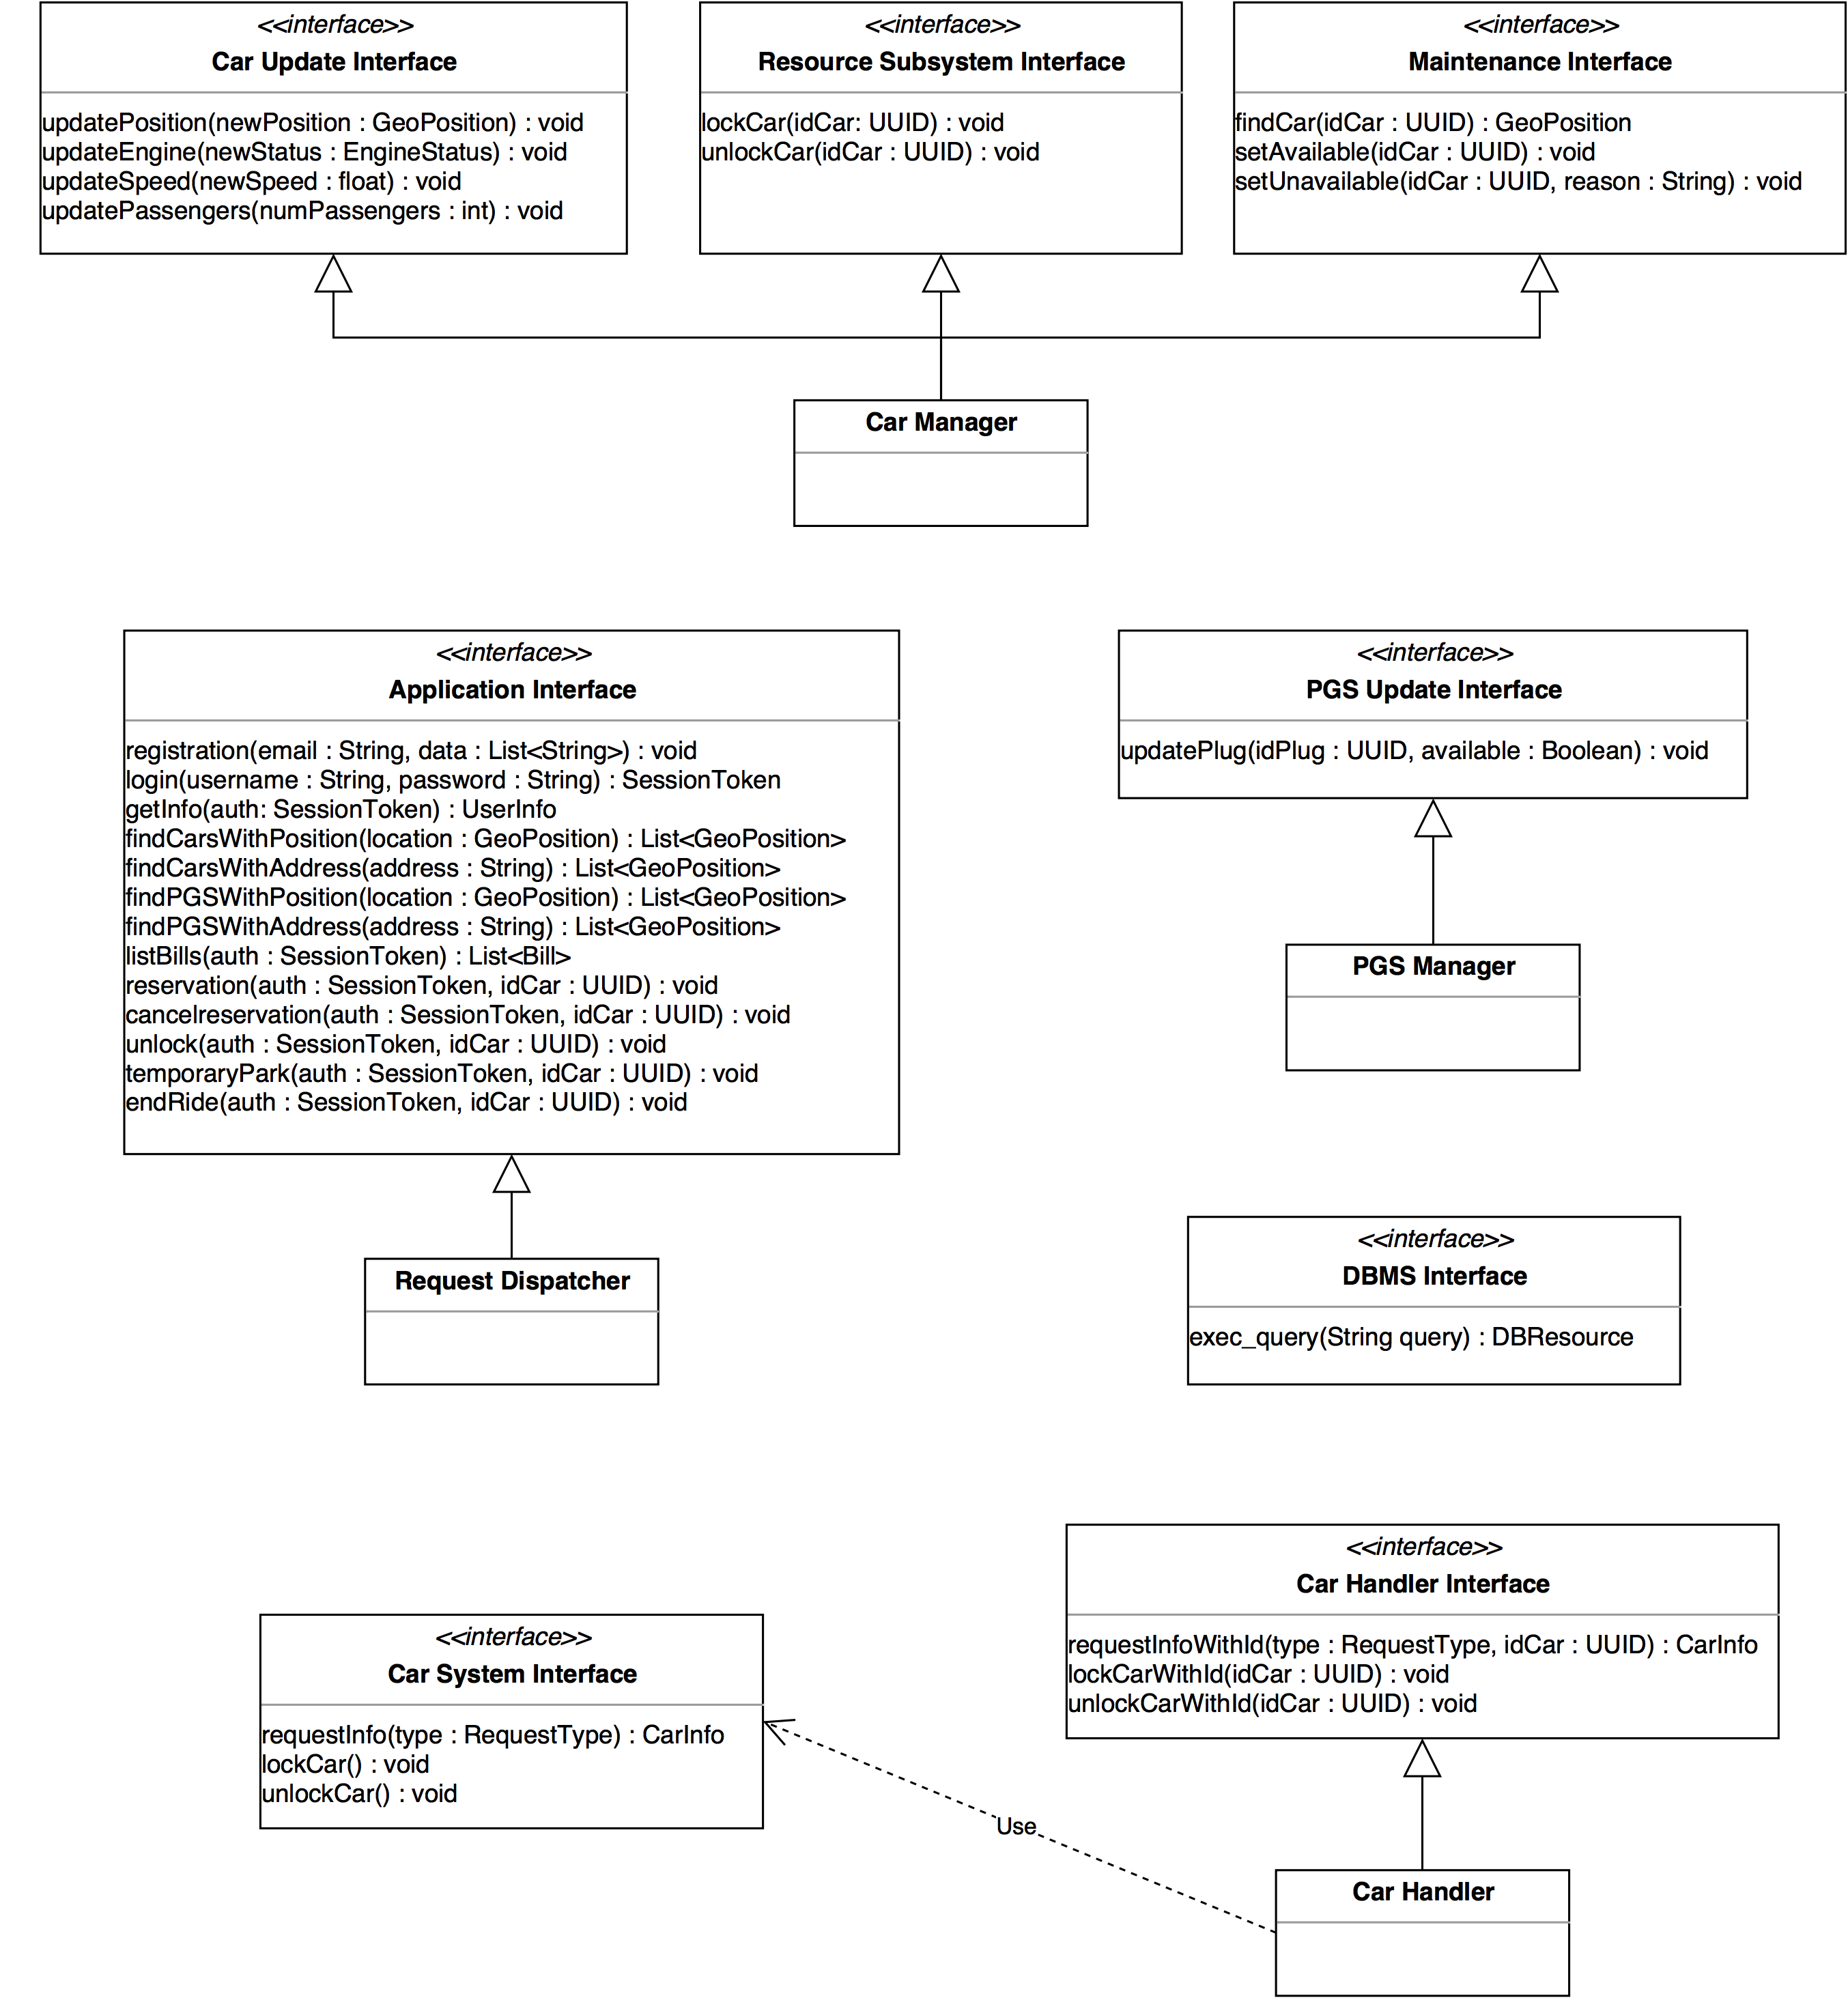
\includegraphics[width=450pt]{comp_interfaces.png}
	}
	\caption{Component Interfaces}
	\label{compinterfaces}
\end{figure}

\subsection{Selected Architectural Styles and Patterns}

% Architecture Overall?

\subsubsection{Protocols}
% rest?

\subsubsection{Patterns}
% mvc
% facade
% client-server
% event-driven architecture
% adapter?

\subsection{Other Design Decisions}

\newpage

\section{Algorithm Design}

% "Java-like pseudo-code"

\subsection{Discount calculation}
\makebox[14cm][c]{
	\lstinputlisting{Discounts.java}
}
\newpage
\subsection{Finding a station for the Money Saving Option}

	\lstinputlisting{MoneySavingOption.java}



\newpage

\section{User Interface Design}

\subsection{Mockups}
% rimandare al RASD

\subsection{UX Diagrams}

\subsection{BCE Diagrams}

\newpage

\section{Requirements Traceability}
% i componenti dell'architettura che sono usati per realizzare ogni goal

% dbms e MODEL?
% se sì, replace dbms con model+dbms sulle parti con l'application subsystem

Goals:
\begin{description}
	\item[{[G1]}]{Guests must be able to register as users by choosing a username and providing their personal data, driving license and payment information. They will receive a password at the email address they specified.}
	\begin{itemize}
		\item{Application Subsystem}
		\item{Request Dispatcher}
		\item{Registration Component}
		\item{DBMS}
		\item{Signup API}
		\item{Driving Licence API}
	\end{itemize}
	\item[{[G2]}]{Users must be able to login with the username/email inserted and the password received on registration.}
	\begin{itemize}
		\item{Application Subsystem}
		\item{Request Dispatcher}
		\item{Login Component}
		\item{DBMS}
	\end{itemize}
	\item[{[G3a]}]{Users must be able to find the location and battery charge of all the available cars within a certain distance from their current location.}
	\begin{itemize}
		\item{Application Subsystem}
		\item{Request Dispatcher}
		\item{Car Search Component}
		\item{Maps API}
		\item{DBMS}
	\end{itemize}
	\item[{[G3b]}]{Users must be able to find the location and battery charge of all available cars around a specified location.}
	\begin{itemize}
		\item{Application Subsystem}
		\item{Request Dispatcher}
		\item{Car Search Component}
		\item{Maps API}
		\item{DBMS}
	\end{itemize}
	\item[{[G4]}]{Users must be able to reserve a car for up to one hour before they pick it up. If they don't take the car before the time expires they are charged a fixed fee of 1 EUR.}
	\begin{itemize}
		\item{Application Subsystem}
		\item{Request Dispatcher}
		\item{Reservation Manager}
		\item{Payment Component}
		\item{DBMS}
	\end{itemize}
	\item[{[G5]}]{Users must be able to cancel a reservation if they decide to not actually use the car.}
	\begin{itemize}
		\item{Application Subsystem}
		\item{Request Dispatcher}
		\item{Reservation Manager}
		\item{DBMS}
	\end{itemize}
	\item[{[G6]}]{A user that reaches a car reserved by them must have a way to tell the system they’re nearby, so that the system unlocks the car and the user may enter.}
	\begin{itemize}
		\item{Application Subsystem}
		\item{Request Dispatcher}
		\item{Unlocking Component}
		\item{Resource Management Subsystem}
		\item{Car Manager}
		\item{Car Handler}
		\item{Car Internal System}
		\item{DBMS}
	\end{itemize}
	\item[{[G7]}]{The system must charge the user who reserved the car from the moment the engine is ignited after unlocking it. The user is charged for a given	amount of money per minute.}
	\begin{itemize}
		\item{Car Internal System}
		\item{Resource Management Subsystem}
		\item{Car Manager}
		\item{DBMS}
	\end{itemize}
	\item[{[G8]}]{The system must allow the user to see the amount they’re being charged through a screen on the car.}
	\begin{itemize}
		\item{Car Application}
		\item{Application Subsystem}
		\item{Request Dispatcher}
		\item{Ride Manager}
		\item{DBMS}
	\end{itemize}
	\item[{[G9]}]{The system must stop charging the user as soon as the car is parked in a safe area and the user exits the car notifying the system that they ended their ride.}
	\begin{itemize}
		\item{Car Internal System}
		\item{Resource Management Subsystem}
		\item{Car Manager}
		\item{Application Subsystem}
		\item{Request Dispatcher}
		\item{Ride Manager}
		\item{Payment}
		\item{Payment API}
		\item{DBMS}
	\end{itemize}
	\item[{[G10]}]{Users must be able to leave a car without losing the reservation by informing the system that they’re only temporarily parking; in this case the system continues on charging the user. The user should be able to end the ride without coming back to the car if they so choose.}
	\begin{itemize}
		\item{Application Subsystem}
		\item{Request Dispatcher}
		\item{Parking Component}
		\item{DBMS}
	\end{itemize}
	\item[{[G11]}]{The system must lock the car automatically after the user exits the car.}
	\begin{itemize}
		\item{Resource Management Subsystem}
		\item{Car Manager}
		\item{Car Handler}
		\item{Car Internal System}
	\end{itemize}
	\item[{[G12]}]{The system must provide a money saving option to the user, proposing a suitable power grid station near the user’s final destination. The user will get a discount if they park the car there and plug it in the power grid.}
	\begin{itemize}
		\item{Application Subsystem}
		\item{Request Dispatcher}
		\item{PGS Search Component}
		\item{Maps API}
		\item{DBMS}
		\item{PGS Internal System}
		\item{PGS Manager}
	\end{itemize}
	\item[{[G13]}]{The stations proposed by the system with the money saving option must be chosen in a way that ensures a uniform distribution of cars in the city.//
		---}
	\item[{[G14]}]{The system must apply a discount of 10\% on the last ride if the user took at least two other passengers onto the car.}
	\begin{itemize}
		\item{Car Internal System}
		\item{Resource Management Subsystem}
		\item{Car Manager}
		\item{DBMS}
		\item{Application Subsystem}
		\item{Ride Manager}
		\item{Payment Component}
	\end{itemize}
	\item[{[G15]}]{The system must apply a discount of 20\% on the last ride if the car is left with more than 50\% of remaining battery charge.}
	\begin{itemize}
		\item{Car Internal System}
		\item{Resource Management Subsystem}
		\item{Car Manager}
		\item{Application Subsystem}
		\item{Ride Manager}
		\item{Payment Component}
		\item{DBMS}
	\end{itemize}
	\item[{[G16]}]{The system must apply a discount of 30\% on the last ride if the car is left at special parking areas where they can be recharged, and the user takes care of plugging the car into the power grid.}
	\begin{itemize}
		\item{Car Internal System}
		\item{Resource Management Subsystem}
		\item{Car Manager}
		\item{Application Subsystem}
		\item{Request Dispatcher}
		\item{Ride Manager}
		\item{Payment Component}
		\item{PGS Internal System}
		\item{PGS Manager}
		\item{DBMS}
	\end{itemize}
	\item[{[G17]}]{The system must charge 30\% more if the car is left at more than 3 km from the nearest power grid station or with less than 20\% remaining battery charge.}
	\begin{itemize}
		\item{Car Internal System}
		\item{Resource Management Subsystem}
		\item{Car Manager}
		\item{Application Subsystem}
		\item{Request Dispatcher}
		\item{Ride Manager}
		\item{Payment Component}
		\item{Maps API}
		\item{DBMS}
	\end{itemize}
	\item[{[G18]}]{Users with outstanding bills cannot have access to the cars and reservations until the bills are paid.}
	\begin{itemize}
		\item{Application Subsystem}
		\item{Request Dispatcher}
		\item{Reservation Manager}
		\item{DBMS}
	\end{itemize}
	\item[{[G19]}]{Users with outstanding bills should have a way to pay them.}
	\begin{itemize}
		\item{Application Subsystem}
		\item{Request Dispatcher}
		\item{Payment}
		\item{DBMS}
	\end{itemize}
	\item[{[G20]}]{Available cars should actually be available to the user and in good conditions (i.e. not dirty, damaged, and/or with low battery).}
	
	%%%%%%% REPORTING %%%%%%%%%%%%%%
	
\end{description}


\newpage

\section{Effort Spent}

\newpage

\section{Revisions}

\subsection{Changelog}
\begin{itemize}
  \item{}
\end{itemize}
\end{document}
